\chapter{Teória neurónových sietí}\label{chap:theory}

V teoretickej kapitole sa budeme podrobnejšie venovať neurónových sieťam bez cyklov. Vysvetlíme čo je základom takýchto sietí tým, že uvedieme princíp, podľa ktorého sa siete rozhodujú a spôsob akým sa učia. Neskôr sa podrobnejšie venujeme konvolučným neurónovým sieťam. Uvádzame ich štruktúru a špecifické vlastnosti. Informácie boli čerpané predovšetkým z prednášok zo Stanford University \cite{SF} a z kníh \cite{RosinPaulL2019RIAa, Goodfellow-et-al-2016}. 

\section{Úvod do neurónových sietí}

Neurónové siete, sú podskupinou strojového učenia a jadrom algoritmov hlbokého učenia. Ich názov a štruktúra sú často prirovnávané k ľudskému mozgu, pretože pripomínajú spôsob, akým si biologické neuróny navzájom signalizujú procesy \cite{Shanmuganathan2016}. Umelá neurónová sieť bez cyklov sa v angličtine označuje aj ako \textit{feed forward neural network (FNN)}. Je tvorená neurónmi, ktoré sa skladajú do vrstiev. Neuróny v susedných vrstvách sú medzi sebou spojené jedným smerom a podobne ako biologický neurón nesú číselnú hodnotu. 

Na prvú, vstupnú vrstvu sú prenesené údaje, ktoré vchádzajú do siete. Do neurónovej siete môžu ísť obrázky, zvuk a prakticky ľubovoľné dáta, ktoré sa dajú vyjadriť číselne. V tejto práci sa budeme zaujímať výhradne o obrázkové vstupy a videá. Neuróny zo vstupnej vrstvy sú ďalej prepojené s jednou, alebo viacerými skrytými vrstvami nasledujúcimi po sebe. Posledná skrytá vrstva sa spája s výstupnou vrstvou. Neuróny vo výstupnej vrstve nesú výsledok vypočítaný zo vstupných údajov. Na obrázku \ref{img:network} je každý neurón v susednej vrstve prepojený so všetkými neurónmi z predchádzajúcej vrstvy. To vo všeobecnosti nemusí byť pravidlom, pretože môžu existovať také siete, kedy sa niektoré spojenia neurónov úmyselne prerušia \cite{DettmersTim2019SNfS}. 
\\
\begin{figure}[ht]
    \centering
    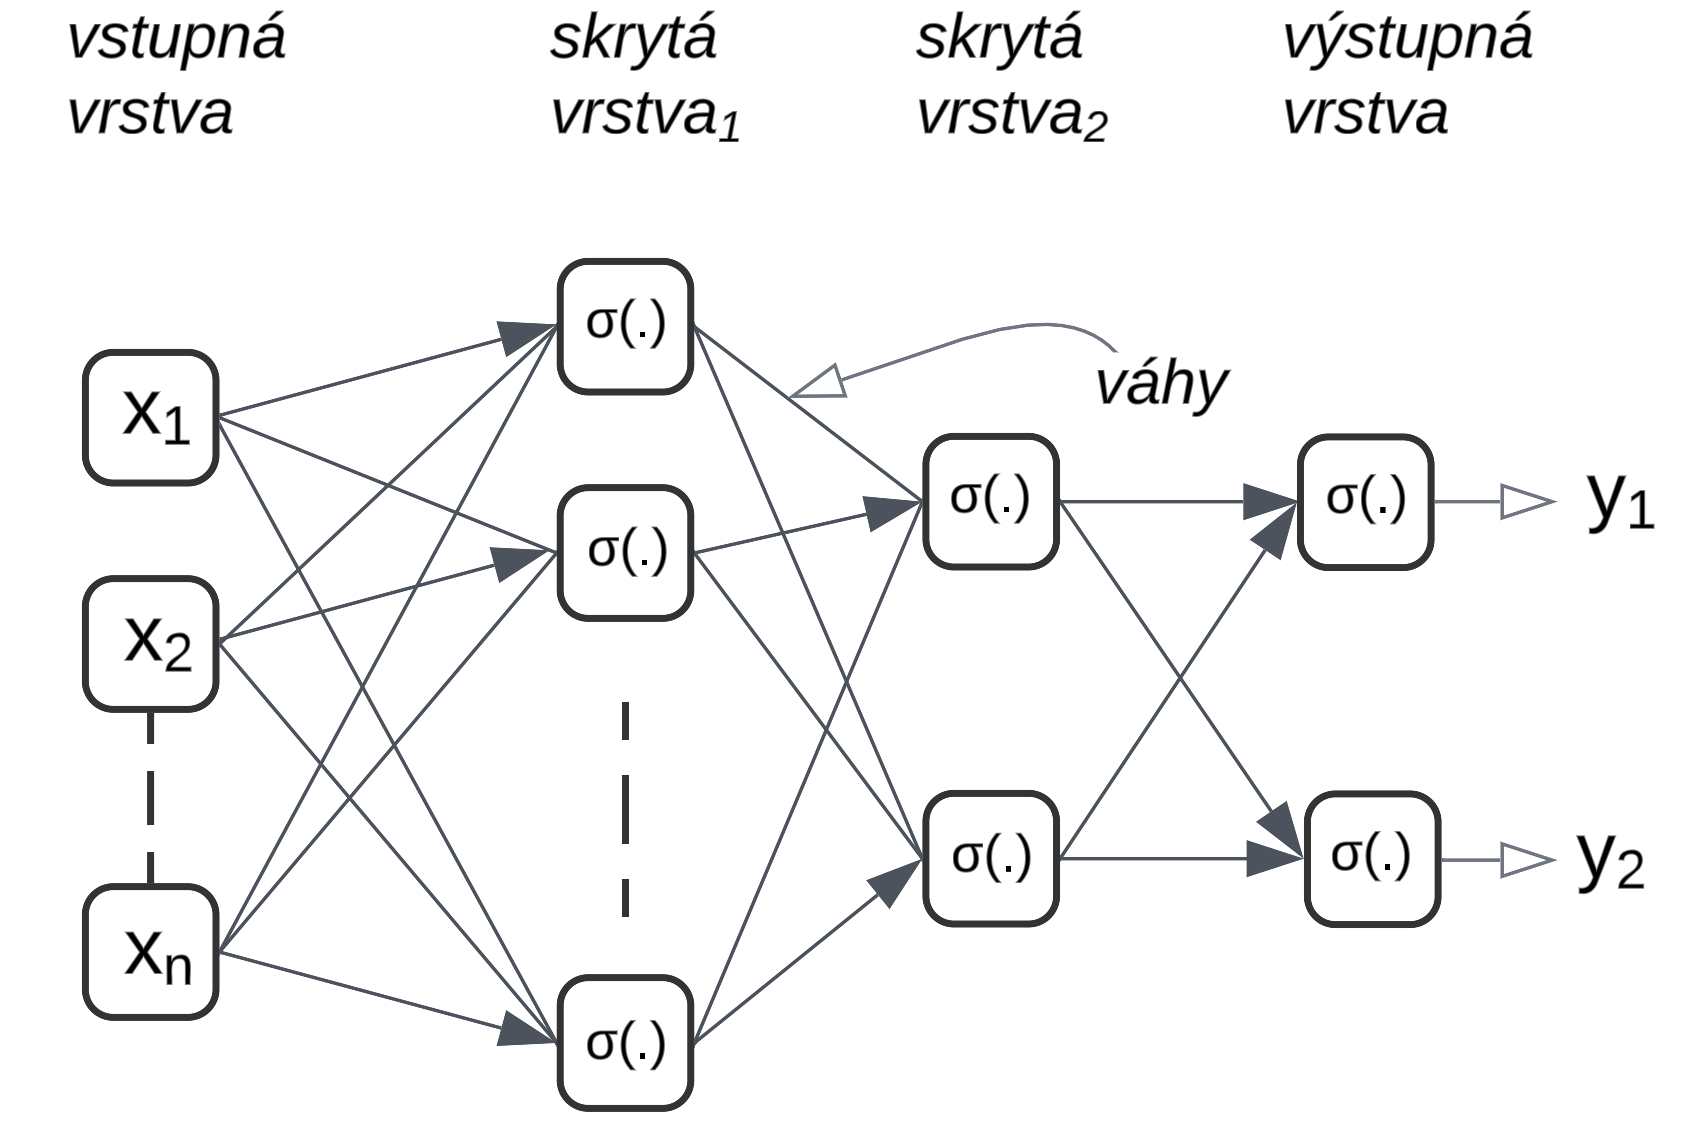
\includegraphics[width=.6\textwidth]{images/02/mynn.png}
    \caption{Neurónová sieť tvorená z dvoch skrytých vrstiev, \begin{math}\sigma(.)\end{math} symbolizuje číselnú hodnotu pre neurón. }
    \label{img:network}
\end{figure}

Vstupom siete je vektor \begin{math}x\end{math}, ktorý je spojený s neurónmi v prvej vrstve. Spojenia medzi neurónmi sa nazývajú váhy. Na základe neurónov a váh sa počítajú hodnoty neurónov v nasledujúcej vrstve. Matematické vyjadrenie pre získanie hodnôt neurónov v nasledujúcej vrstve je opísané formulou:

\begingroup
\large
\begin{equation}a^{i+1} = \sigma \left ( \sum_{j=1}^{n^i} w_{j}^i a_{j}^i + bias^{i+1} \right ) \end{equation}
\endgroup
 
kde \begin{math}n^{i}\end{math} je počet spojení s neurónom, \begin{math}a^{i}\end{math} sú hodnoty spojených neurónov z predchádzajúcej vrstvy a \begin{math}w^{i}\end{math} sú hodnoty spojení. Do výpočtu zasahuje ešte hodnota \begin{math}bias\end{math}, ktorá sa vzťahuje na počítaný neurón. Každý neurón je v zásade funkčnou hodnotou aktivačnej funkcie \begin{math}\sigma\end{math} po násobení matíc a pripočítaní hodnoty \begin{math}bias\end{math}. Podobne ako biologický neurón dokáže aktivovať svojho suseda, tak aj pre umelý neurón platí, že čím má väčšiu hodnotu, tým viac ovplyvňuje hodnotu neurónu v susednej vrstve.

% formula: https://youtu.be/aircAruvnKk?t=905
% bias: https://youtu.be/rJmBhnLzjOM?t=133

Aktivačné funkcie zohrávajú dôležitú úlohu v neurónových sieťach, tým že zabraňujú lineárnemu počítaniu. To umožňuje neurónovým sieťam vyvíjať zložité reprezentácie, ktoré by nebolo možné dosiahnuť pomocou jednoduchého lineárneho modelu. Známe aktivačné funkcie sú napríklad \textit{Sigmoid} \cite{sigmoid}, \textit{Rectified Linear Units (ReLU)} \cite{relu} a jej variácie. ReLU je často používaná vďaka jednoduchej implementácii nelineárnej transformácie a dobrému výkonu pri rôznych úlohách. Zachováva iba pozitívne prvky a všetky negatívne prvky nastaví na nulovú hodnotu. Variácie ReLU zachovávajú určitú časť informácie aj pre negatívne prvky. Na obrázku \ref{img:rr} je zobrazený priebeh ReLU s parametrom a bez parametra. Parameter pre negatívnu časť nie je konštantný, ale je adaptívny pre naučenie \cite{prelu}.
\\
\begin{figure}[ht]
    \centering
    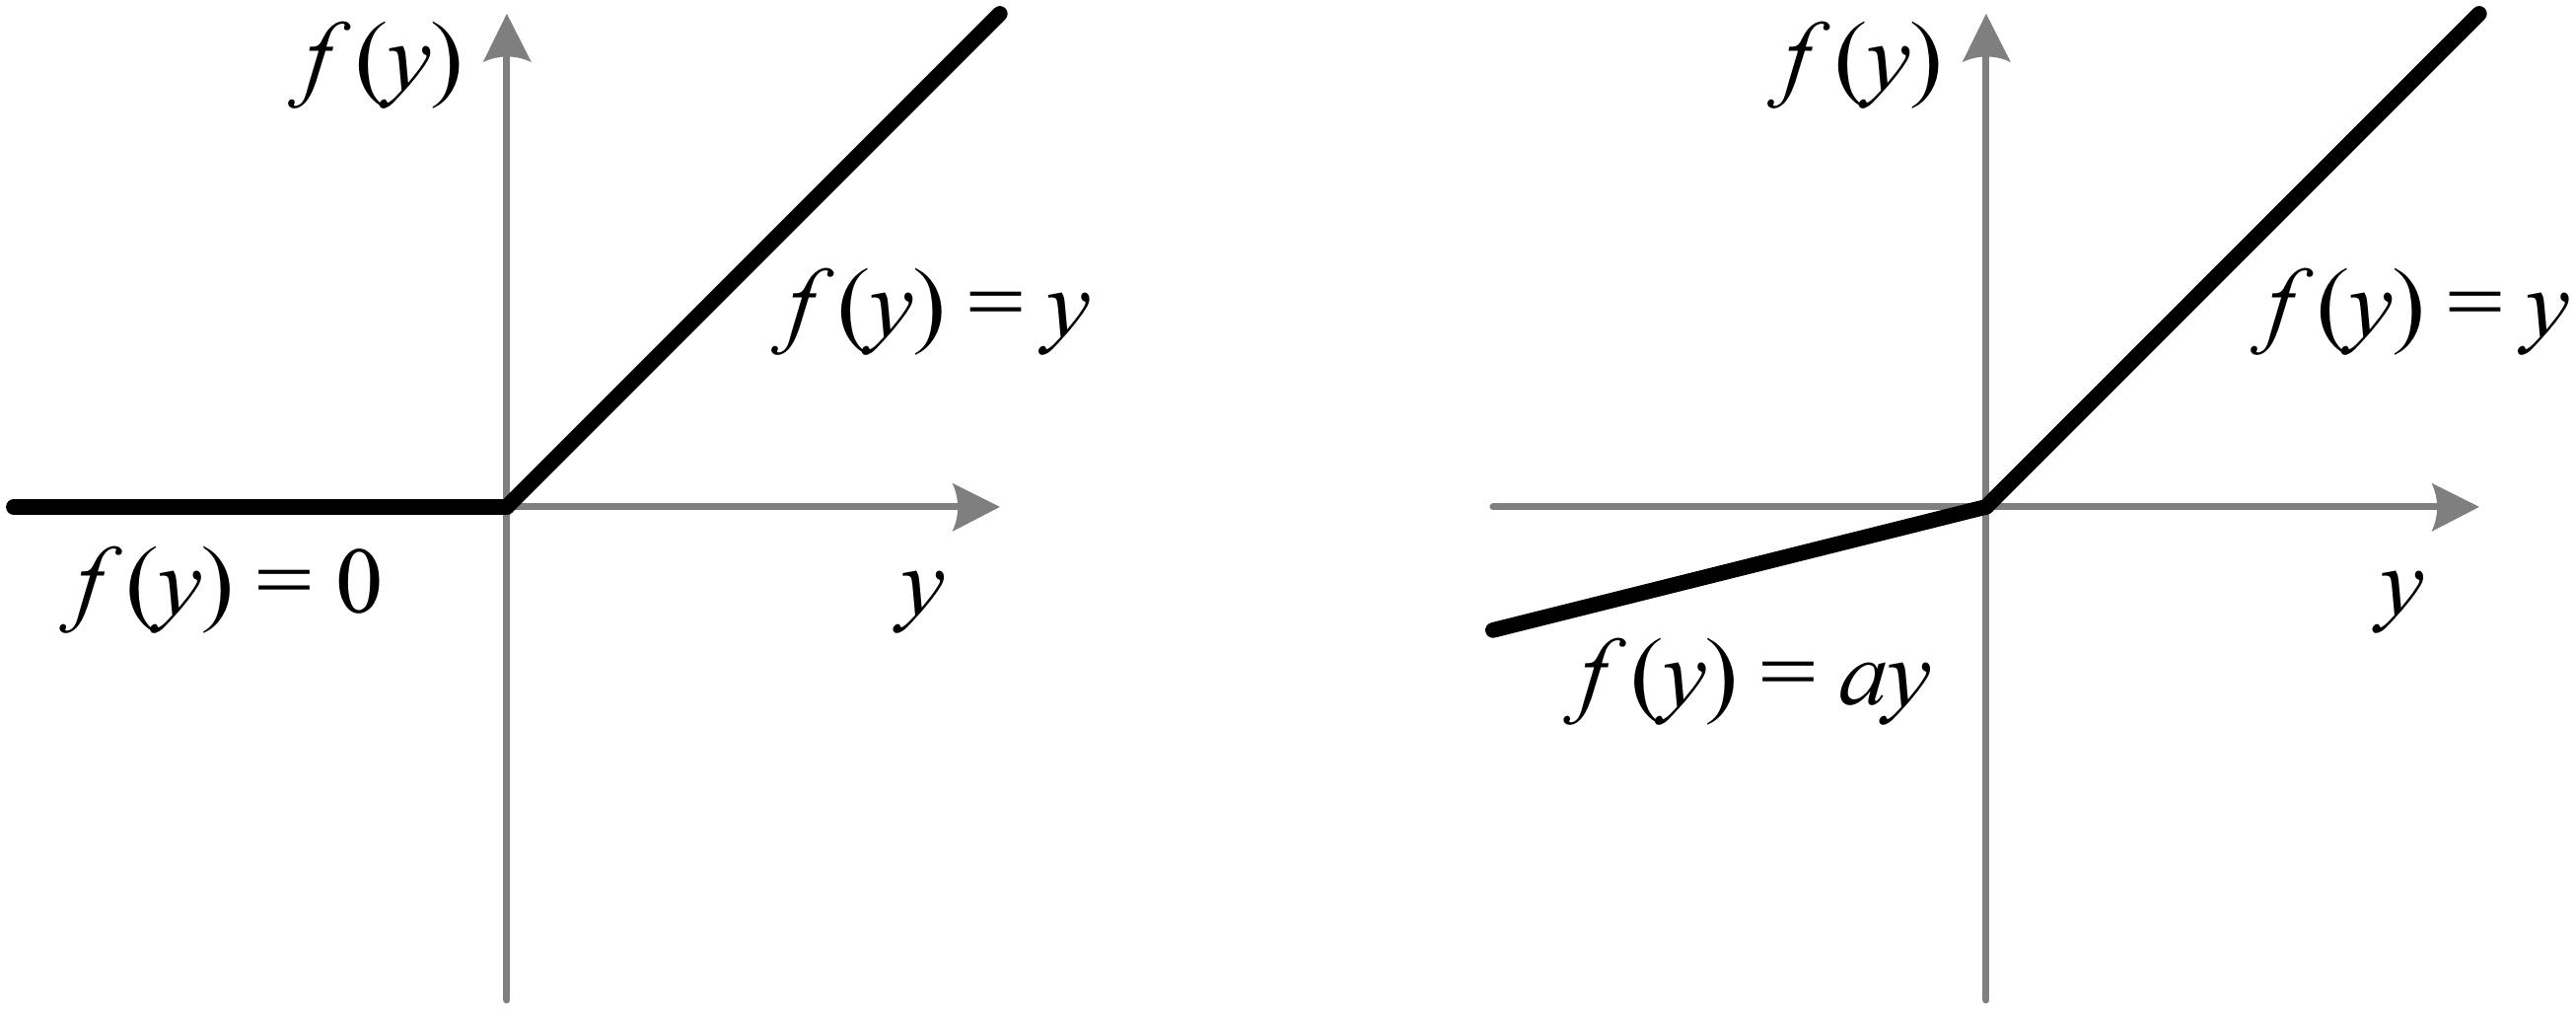
\includegraphics[width=.6\textwidth]{images/02/relu_prelu.png}
    \caption{Porovnanie aktivačnej funkcie ReLU (naľavo) a jej variácie PReLU (napravo) \cite{prelu}.}
    \label{img:rr}
\end{figure}

\section{Princíp učenia}

Neurónové siete využívajú heuristický spôsob učenia. Učenie sa vzťahuje na proces úpravy váh tak, aby boli špecializované vykonávať konkrétnu úlohu. Učenie by nebolo možné bez vstupných údajov, od ktorých sú neurónové siete závislé. Teoreticky platí, že čím viac je k dispozícií kvalitných dát, tým má sieť väčší potenciál dosiahnuť lepšie výsledky pri učení. Keď je neurónová sieť natrénovaná, môže byť použitá na predpovedanie informácií o nových vstupných údajoch, ktoré počas učenia nevidela. Výkon neurónovej siete na týchto nových údajoch je mierou toho, ako dobre je sieť naučená vykonávať svoju úlohu.

\subsection{Učenie s pomocou učiteľa}
Prístup učenia s pomocou učiteľa sa spolieha na správne označené dáta pri riešení úloh akým sú klasifikácia, lokalizácia, detekcia a segmentácia. Ak ide o trénovanie siete za účelom klasifikácie obrázka, tak je každý obrázok označený informáciou, do ktorej triedy patrí. Ak ide o detekciu objektov, tak okrem informácie o výskyte konkrétneho objektu sa označuje príslušný bounding box, ktorý vymedzuje jeho polohu. Počiatočné váhy medzi uzlami sú vygenerované náhodne, prípadne sa zvyknú použiť už natrénované váhy z blízkej sady obrázkov pre lepší nástup trénovania. Spôsob, kedy sa použijú natrénované váhy sa nazýva prenášané učenie (\textit{transfer learning}). 

Postup akým sa sieť učí, môžeme demonštrovať na úlohe klasifikácie obrázkov do troch tried. Údaje z obrázka sa prenesú na vstupnú vrstvu a postupným počítaním prechádzajú každou vrstvou. Na poslednej vrstve každý neurón reprezentuje jednu triedu klasifikácie. Hodnoty pre výstupné neuróny môžeme určiť napríklad pomocou \textit{Softmax} funkcie. Pri tejto konkrétnej funkcii sa dá výstup chápať ako pravdepodobnosť, podľa ktorej je sieť rozhodnutá klasifikovať obrázok do konkrétnej triedy. Sieť klasifikuje vstupný obrázok triedou, ktorá prislúcha neurónu s najvyššou hodnotou na výstupnej vrstve. Súčet pravdepodobností je rovný číslu 1. Najlepší možný výsledok by vyzeral tak, že neurón označujúci správnu triedu by mal hodnotu 1, kým ostatné neuróny hodnotu 0. Takýto výsledok však nie je pravdepodobný a ani to nie je nutné na dosiahnutie vysokej presnosti klasifikátora.

Počas učenia sa výstup zo siete porovnáva s pôvodným označením obrázka. Porovnanie klasifikácie pomocou možností správne a nesprávne na učenie nestačí. Do úvahy sa berú všetky hodnoty na výstupnej vrstve, z ktorých sa počíta celková chyba klasifikácie podľa stratovej funkcie. Výber stratovej funkcie opäť nie je jednoznačne daný, ale často používanými funkciami sú napríklad \textit{Cross-entropy loss} alebo \textit{Hinge loss} \cite{loss}. Aby sme natrénovali neurónovú sieť na vykonanie úlohy, musíme upraviť váhy takým spôsobom, aby sa zmenšila chyba vypočítaná stratovou funkciou. 

Na zníženie chyby sa využíva proces spätnej propagácie (backpropagation) \cite{bp}, pomocou ktorého sa mierne zvyšujú alebo znižujú váhy od výstupných vrstiev smerom dozadu podľa vypočítaného gradientu. Gradient descent je iteračný algoritmus, ktorý hľadá lokálne minimum stratovej funkcie pomocou gradientu, ktorého smer otočí a podľa zvoleného kroku sa posunie. Opakovaným procesom sa hodnota stratovej funkcie znižuje spolu so zmenou váh medzi uzlami, až kým je nie dosiahnutá požadovaná presnosť alebo kým nie sú splnené iné podmienky na ukončenie. Inou podmienkou okrem presnosti môže byť dosiahnutie pevného počtu iterácií alebo situácia keď, chyba sa po viacerých iteráciách za sebou nezmenšuje.

Gradient descent hľadá minimum iba v blízkosti aktuálneho bodu na ploche stratovej funkcie. Často je výpočtovo nemožné hľadať globálne minimum na celom povrchu stratovej funkcie. Okrem toho niektoré stratové funkcie môžu mať viacero globálnych miním alebo dokonca žiadne globálne minimum. Ak má stratová funkcia viac lokálnych miním, gradient descent môže konvergovať k suboptimálnemu riešeniu. Pokiaľ lokálne minimum nemá často vysokú stratu, tak ide o prijateľné riešenie. To či bolo nájdených veľa lokálnych miním s vysokou stratou zostáva aktívnou oblasťou výskumu, ale odborníci si myslia, že pre dostatočne veľké neurónové siete má väčšina lokálnych miním nízku stratu a že nie je dôležité nájsť skutočné globálne minimum \cite{Goodfellow-et-al-2016}. Obrázok \ref{img:gradient} zobrazuje jednoduchú funkciu v dvojrozmernom priestore. V skutočnom prípade sieť pracuje s oveľa zložitejšou funkciou.
\\
\begin{figure}[h]
    \centering
    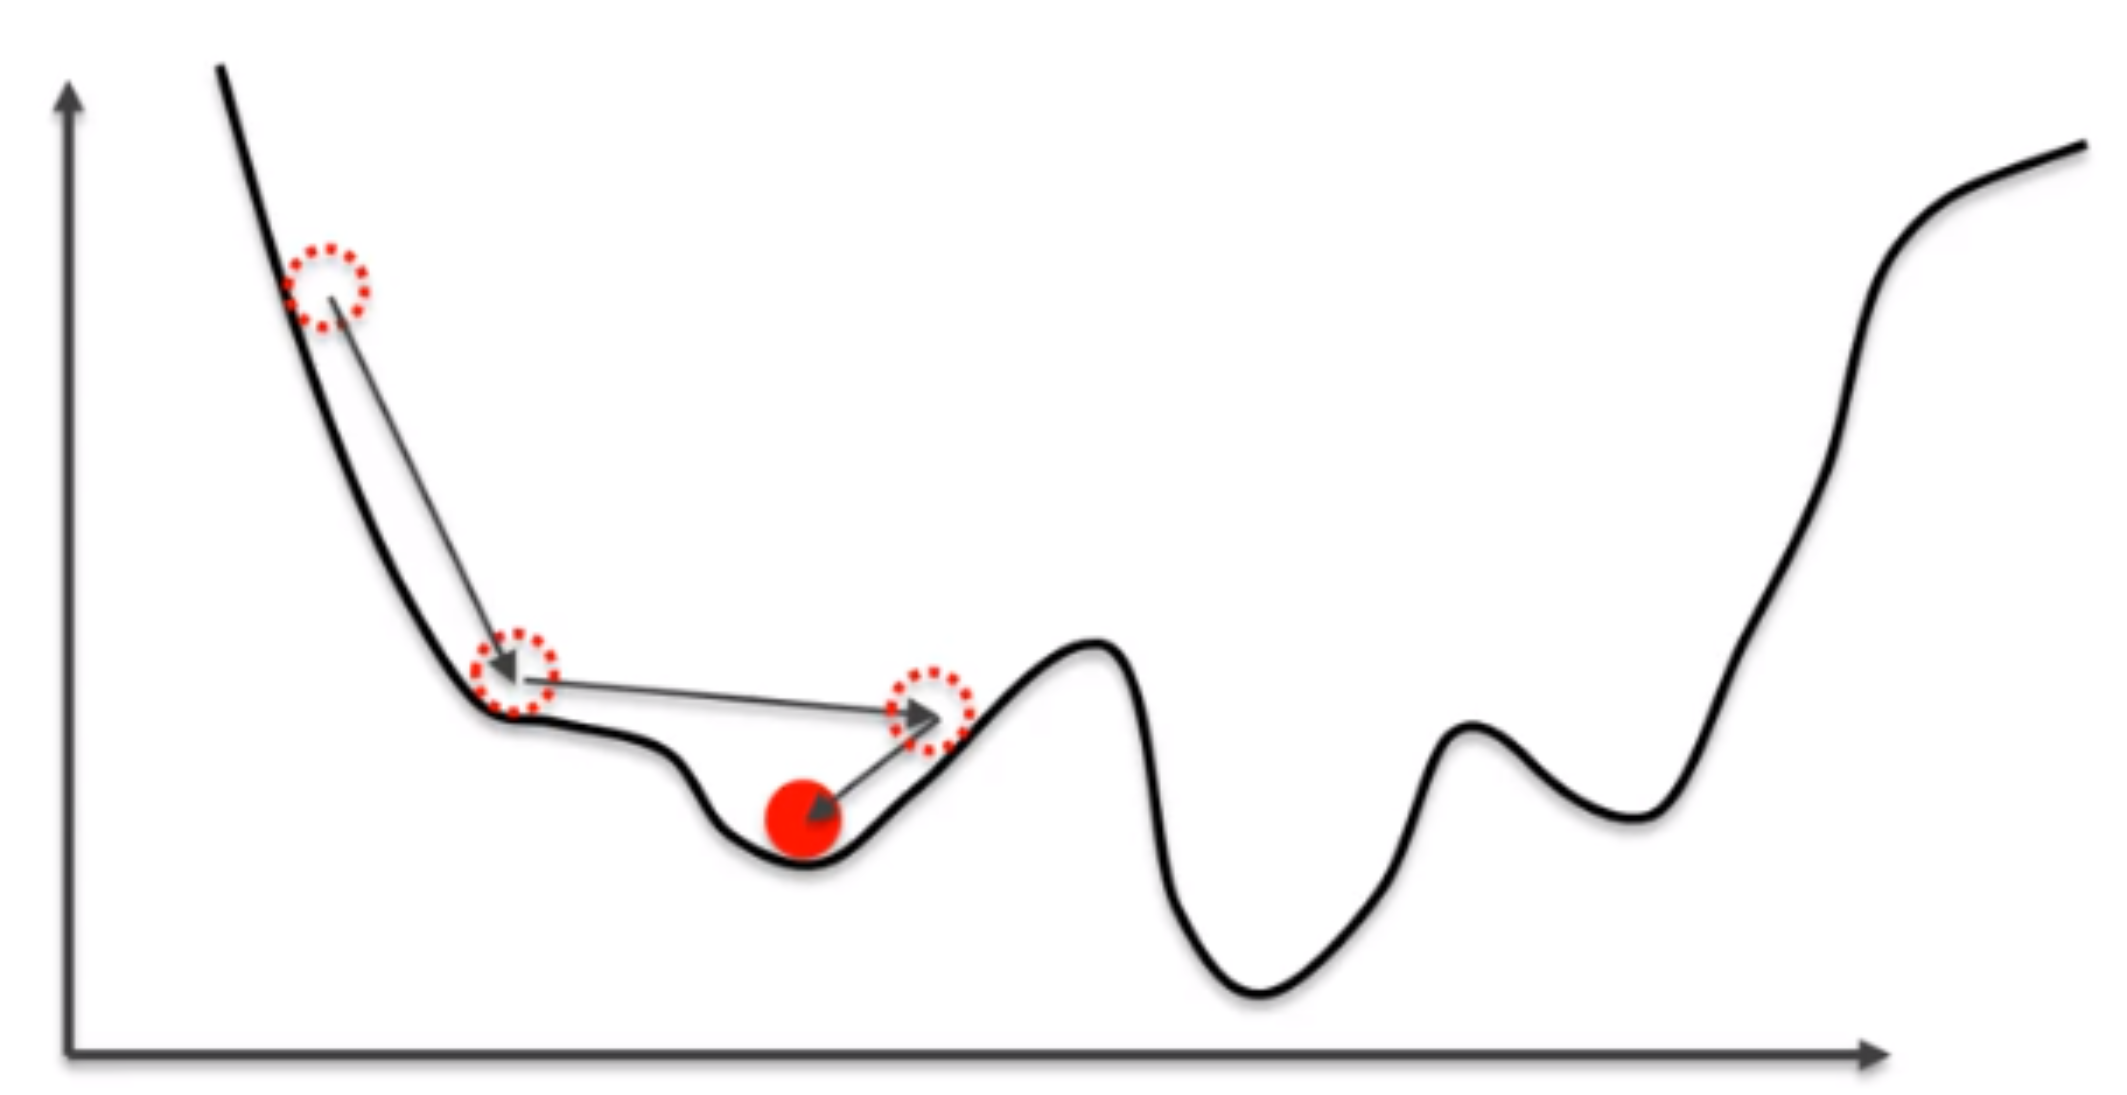
\includegraphics[width=.5\textwidth]{images/02/grad.png}
    \caption{Zjednodušená postupnosťou krokov optimalizačného algoritmu hľadajúc minimum funkcie. \cite{grad}}
    \label{img:gradient}
\end{figure}

To čo sme opísali je len základný zjednodušený princíp učenia. V skutočnom prípade je učenie komplikovanejšie. Je ovplyvnené pomocou ďalších techník a hyper-parametrov, ktoré sa dajú obmieňať, čo prináša rôzne výsledky pri trénovaní. Medzi hyper-parametre patrí spomenutý krok učenia, veľkosť dávky, počet epoch, sila regularizácie a mnohé iné. Ich definície ponúkajú hlbší pohľad do vnútra fungovania neurónovej siete.

Napokon je dôležité, aby dataset obsahoval veľa obrázkov, ktoré sú dobre označené. Objekty, ktoré chceme detegovať by mali mať dostatočnú diverzitu a približne rovnakú distribúciu. Dataset je spravidla rozdelený do troch častí. Trénovacia sada je najväčšia, aby mala sieť čo najviac dát. Validačná sada je oddelená od trénovacej sady a používa sa na overenie výkonnosti modelu počas trénovania. Model sa učí na trénovacej sade a súčasne sa po každej vykonanej epoche vykonáva hodnotenie modelu na validačnej sade. Hlavnou myšlienkou validačnej sady je zabrániť prehnanému trénovaniu modelu. Testovacia sada slúži na určenie toho ako dobre sa neurónovú sieť podarilo natrénovať.

\section{Konvolučné neurónové siete}

Bežné neurónové siete nepracujú dobre s väčšími údajmi. Napríklad pre obrázky veľkosti 32x32 pixlov s troma farebnými kanálmi má jeden plne pripojený neurón v prvej skrytej vrstve 3072 váh (32x32x3). Pre väčší obrázok, napríklad 420x420x3 by mal jeden neurón 529 200 spojení, ktorých trénovanie vyžaduje veľa výpočtového výkonu.

Cieľom konvolučných neurónových sietí (CNN) je zmenšiť obrázky tak, aby sa dali ľahšie spracovať bez straty príznakov, ktoré sú dôležité pre čo najpresnejší výsledok. V porovnaní s bežnými neurónovými sieťami majú konvolučné siete zmenenú štruktúru vrstiev. Zahŕňajú tri typy vrstiev: konvolučnú vrstvu, pooling vrstvu a plne prepojenú vrstvu.

\subsection{Konvolučná vrstva}

Konvolučná vrstva je dominantnou časťou konvolučných neurónových sietí. V prípade CNN je konvolúcia použitá na získanie mapy príznakov zo vstupného obrázka. Použitie konvolučných vrstiev sa ukázalo ako efektívne pri rozpoznávaní obrazu, detekcii objektov a iných úlohách počítačového videnia. Formálne je konvolúcia v kontexte CNN definovaná nasledujúcim vzorcom, kde K je filter (kernel) a I vstupný obraz \cite{cnn-intro}:

\begingroup
\large
\begin{equation}
(I*K)_{i,j} = \sum_{m} \sum_{n} I_{i-m, j-n} K_{m,n}
\end{equation}
\endgroup

Filter postupne prechádza cez celý vstup a vykoná konvolúciu v každom jeho okolí. Na obrázku \ref{img:conv} je vstup s rozmermi 7x7x3, na ktorý sa postupne aplikuje 128 filtrov s rozmerom 3x3x3. Filter môže mať rôzne rozmery, ale najpoužívanejšie sú 1x1, 3x3 a 5x5. Tretí rozmer je totožný s hĺbkou na vstupe. Po konvolúcii filtra vždy dostaneme hĺbku 1, čo znamená, že výstup v ukážke bude mať hĺbku 128. Okrem rozmeru filtra sa určuje aj to, aké nadobúda hodnoty. Napríklad môže isť o filter na vyhľadávanie horizontálnych hrán. Spolu s filtrom treba určiť krok, ktorý hovorí o koľko pixlov sa má posunúť filter po každom výpočte pri prechádzaní vstupným obrázkom. Vstupnému obrázku sa dá pridať vonkajšie ohraničenie. Ohraničenie vytvára dodatočné pixle okolo hraníc vstupu, aby zabránil strate ich informácii. Pre vstup s rozmerom \begin{math}W_1xH_1xD\end{math} je výsledný rozmer \begin{math}W_2xH_2xK\end{math}, kde \begin{math}W_2 = (W_1 - F + 2P)/S + 1, H_2 = (H_1 - F + 2P)/S + 1\end{math} pre P počet pixlov ohraničenia, S veľkosť kroku, F rozmer filtra a K počet filtrov.

\begin{figure}[ht]
    \centering
    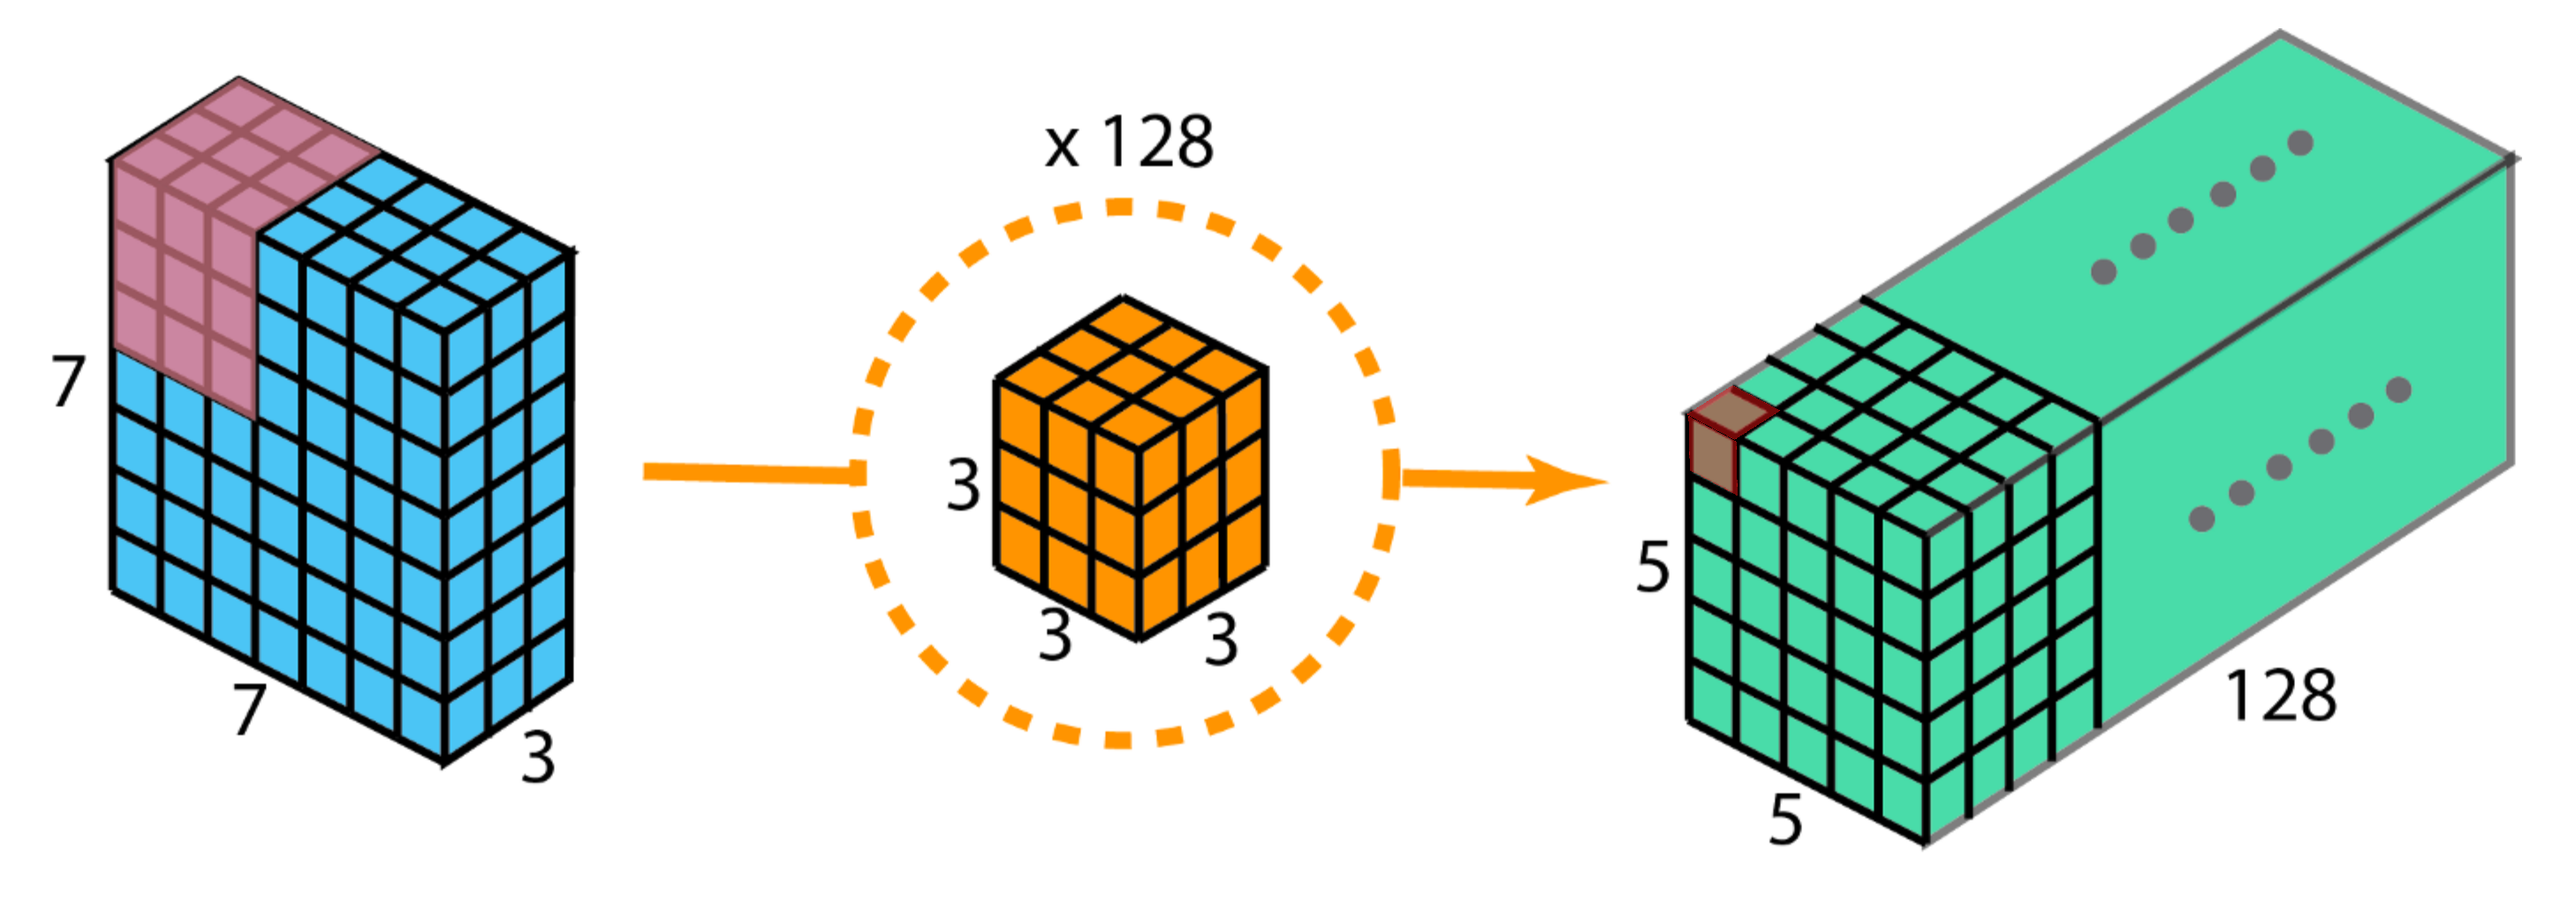
\includegraphics[width=.7\textwidth]{images/02/filters2.png}
    \caption{Ukážkové naznačenie konvolúcie. Červenou farbou je naznačený vstup a výstup pre prvý konvolučný výpočet \cite{filters}. }
    \label{img:conv}
\end{figure}

\subsection{Pooling vrstva}

Po konvolučnej vrstve býva často do architektúry nasadená pooling vrstva. Je užitočná na zmenšenie rozmerov príznakovej mapy, čím je výpočet ešte efektívnejší. Pooling vrstva má nastaviteľnú veľkosť filtra, ktorý je zvyčajne 2x2 alebo 3x3 pixlov a krok. Funkcia, ktorou sa počíta výstup môže byť opäť rôzna. Najbežnejšie je to maximálna hodnota z okolia, ale existujú aj ďalšie často používané funkcie ako je počítanie priemeru alebo združovanie podľa normy L2. \cite{cnn-intro}. Pre vstup s rozmerom \begin{math}W_1xH_1xD\end{math} je tentokrát výsledný rozmer \begin{math}W_2xH_2xC\end{math}, kde \begin{math}W_2 = (W_1 - F)/S + 1, H_2 = (H_1 - F)/S + 1\end{math}. To znamená, že oproti konvolučnej vrstve ostáva zachovaná hĺbka.

\begin{figure}[ht]
    \centering
    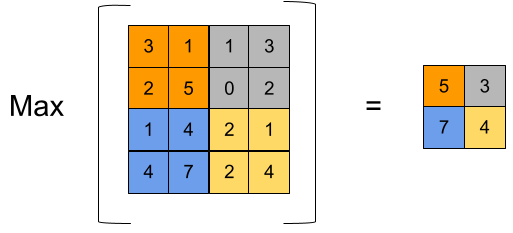
\includegraphics[width=.5\textwidth]{images/02/pooling.png}
    \caption{Vstup a výstup po max-pooling funkcii s veľkosťou filtra 2x2 a krokom 2 \cite{pool}.}
    \label{img:maxpool}
\end{figure}

\subsection{Plne prepojená vrstva}

Po tom čo údaje prejdu cez všetky konvolučné a pooling vrstvy, vstupujú do plne prepojenej vrstvy. Tá je v zásade totožná s neurónovou sieťou, ktorú sme uvádzali v úvode kapitoly. Plne prepojená vrstva dostáva na vstup jednorozmerné údaje, z ktorých je vypočítaný konečný výsledok siete.

\subsection{Existujúce architektúry}

Obrázok \ref{img:lenet} zobrazuje prvú konvolučnú neurónovú sieť, ktorú navrhol Yann LeCun v roku 1998, s názvom LeNet-5. Bola vytvorená na identifikáciu ručne písaných číslic, pričom dosiahla presnosť 98\% \cite{lenet}. Jej vznik určil základnú architektúru konvolučných neurónových sietí.

\begin{figure}[ht]
    \centering
    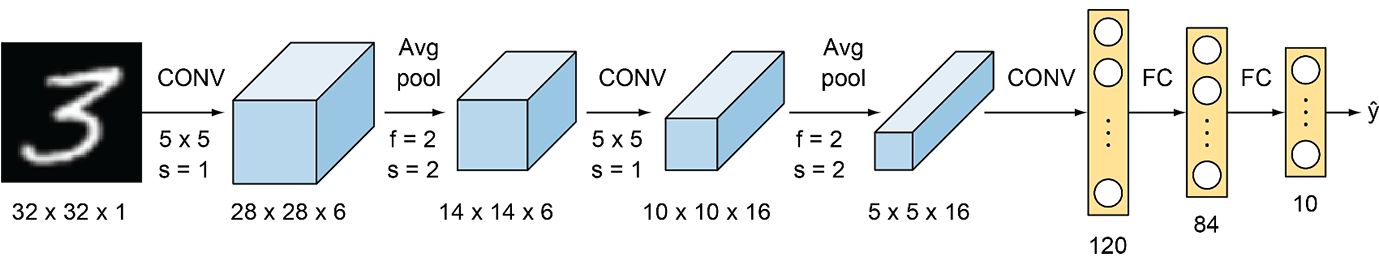
\includegraphics[width=1\textwidth]{images/02/lenet5.png}
    \caption{Náčrt architektúry prvej konvolučnej neurónovej siete LeNet-5 \cite{lenet}.}
    \label{img:lenet}
\end{figure}

Prvou konvolučnou sieťou, ktorá vyhral majstrovstvá súťaže ILSVRC bola sieť AlexNet v roku 2012. Bola vytvorená zo základnej architektúry LeNet-5. Pozostáva z piatich konvolučných vrstiev, troch pooling vrstiev a troch plne prepojených vrstiev, s celkovým počtom 60 miliónov parametrov \cite{AlexNet}. Na testovacej sade ILSVRC chybovosť dosiahla úroveň 15,3\%, s výrazným rozdielom oproti druhému miestu s chybou 26,2\% \cite{ilsvrc}. Úspech siete AlexNet bol spôsobený viacerými vylepšeniami. Napríklad rozšírením trénovacích údajov pomocou úprav originálnych obrázkov, použitím aktivačnej funkcii ReLu, ktorá vtedy nebola bežne používaná a náhodným odstránim spojitých neurónov pomocou regularizačnej metódy \textit{dropout}.

\subsubsection{YOLO}
TODO. (just dummy copy-paste) The first 20 convolution layers of the model are pre-trained using ImageNet by plugging in a temporary average pooling and fully connected layer. Then, this pre-trained model is converted to perform detection since previous research showcased that adding convolution and connected layers to a pre-trained network improves performance. YOLO’s final fully connected layer predicts both class probabilities and bounding box coordinates.

YOLO divides an input image into an S × S grid. If the center of an object falls into a grid cell, that grid cell is responsible for detecting that object. Each grid cell predicts B bounding boxes and confidence scores for those boxes. These confidence scores reflect how confident the model is that the box contains an object and how accurate it thinks the predicted box is.

YOLO predicts multiple bounding boxes per grid cell. At training time, we only want one bounding box predictor to be responsible for each object. YOLO assigns one predictor to be “responsible” for predicting an object based on which prediction has the highest current IOU with the ground truth. This leads to specialization between the bounding box predictors. Each predictor gets better at forecasting certain sizes, aspect ratios, or classes of objects, improving the overall recall score.

One key technique used in the YOLO models is non-maximum suppression (NMS). NMS is a post-processing step that is used to improve the accuracy and efficiency of object detection. In object detection, it is common for multiple bounding boxes to be generated for a single object in an image. These bounding boxes may overlap or be located at different positions, but they all represent the same object. NMS is used to identify and remove redundant or incorrect bounding boxes and to output a single bounding box for each object in the image.

\begin{figure}[ht]
    \centering
    
\includegraphics[width=1\textwidth]{images/placeholder.png}
    \caption{YOLO.}
    \label{img:ch2}
\end{figure}

\section{Výzvy neurónových sietí}
Použitie neurónových sieti mnohokrát prináša veľmi dobré výsledky pre mnohé projekty a úroveň state-of-art sa rokmi zlepšuje. Bohužiaľ mnohé práce narážajú na niekoľko problémov, ktoré bránia dosiahnuť dobrú presnosť neurónovej siete \cite{RosinPaulL2019RIAa}.

\subsubsection{Trénovacie údaje}
Na vytvorenie robustného detektoru objektov, ktorý dokáže prekonať bežné problémy s detekciou, ktoré boli spomenuté v prvej kapitole, treba zabezpečiť, že pre použitý dataset existuje dobrá variácia tréningových dát. Aj napriek tomu, že sa v modernej dobe dáta rýchlo rozrastajú, tak nie vždy sa nájde dostatočne veľký a kvalitný dataset pre konkrétnu problematiku. Niekto musí dáta ručne anotovať a môže sa pri tom dopustiť nekonzistentnému označovaniu alebo iných chýb, čo môže zapríčiniť slabšie výsledky siete, predovšetkým na malom súbore dát.

\subsubsection{Výpočtový čas}
Vo všeobecnosti si trénovanie môže dovoliť trvať dlhý čas, no výpočtový čas je často veľmi dôležitým kritériom výkonu, ktorý môže byť hlavnou požiadavkov pre niektoré aplikácie. Ako príklad sa dajú uviesť časovo kritické aplikácie, akými sú autonómne riadenie a sledovacie systémy, ktoré musia nevyhnutne fungovať v reálnom čase. Iné aplikácie, napríklad náš projekt, si môže dovoliť pomalšie časy výpočtu. Často tak existuje kompromis medzi výpočtovým časom a výkonom siete. Dlhý čas trénovania môže byť v niektorých prípadoch predsa len problém. Nie každý si môže dovoliť dlho čakať na výsledky, prípadne nemá zdroje, ktoré by zvládli natrénovať model v prijateľnom čase alebo s dostatočne veľkými parametrami.

\subsubsection{Podobnosť a variácia trieď}
Objekty, ktoré sa snaží počítač vidieť a rozoznať sa môžu medzi sebou veľmi podobať a napriek tomu byť označené rozdielnymi triedami. Vonkajšia podobnosť môže ľahko spôsobiť nesprávne priradenie triedy objektu. Na druhej strane, jedna trieda môže mať veľmi veľa variácií. Predovšetkým sa to stáva pre objekty vytvorené človekom alebo prírodou. Napríklad na obrázku \ref{img:ch2} vidíme rôzne podoby stoličky, ktoré sa výrazne líšia, ale nemáme problém povedať, že ide o stoličku. Pokiaľ niektorá nezvyčajná podoba stoličky nie je v trénovacích dátach, tak pravdepodobne nebude rozoznaná. Druhá časť obrázku \ref{img:ch2} ukazuje, že aj keď sú objekty z rôznych tried, tak sa môžu veľmi podobať. Napríklad mačka a puma sú si veľmi podobné, ale sú z rôznych tried. Toto môže spôsobiť, že sa mačka označí ako puma alebo naopak.

\begin{figure}[ht]
    \centering
    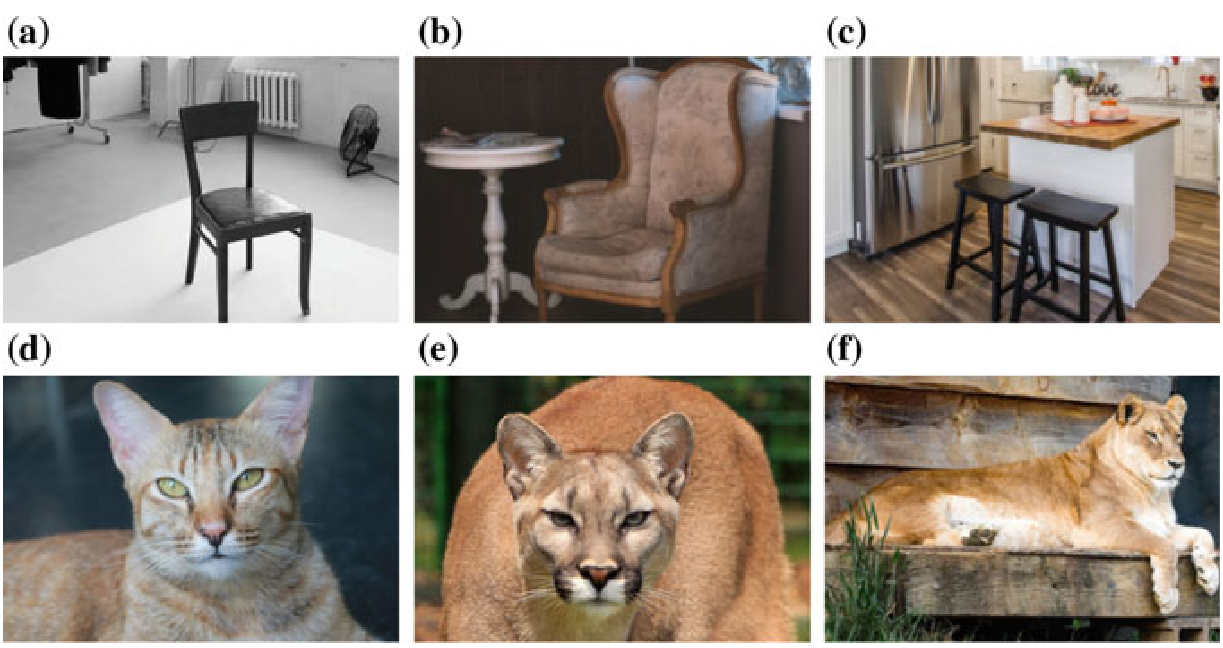
\includegraphics[width=1\textwidth]{images/02/challenge2.png}
    \caption{Príklad variácie vrámci jednej triedy (a–c) a príklad podobnosti medzi triedami (d–f) \cite{RosinPaulL2019RIAa}.}
    \label{img:ch2}
\end{figure}

\subsubsection{Osvetlenie, oklúzia a deformácia}
V neposlednom rade výsledky komplikujú podmienky, pri ktorých je hľadaný objekt zachytený. Osvetlenie môže byť problémom, keď je objekt v scéne príliš tmavý alebo príliš svetlý. Príkladom môže byť autonómne riadenie vozidla, ktoré musí fungovať počas celého dňa, čiže za každých svetelných podmienok a to aj v extrémnych situáciách a pri náhlich zmenách. Oklúzia nastáva, keď objekt nie je viditeľný celý kvôli jeho celému alebo čiastočnému prekrytiu. Deformácia nastáva hlavne pre objekty, ktoré nie sú pevné a tak sa môžu vyskytovať v rôznych neštandardných formách.